\documentclass[11pt,a4paper]{article}
\usepackage[T1]{fontenc}
\usepackage{iftex}
\ifPDFTeX\usepackage[utf8]{inputenc}\fi
\usepackage{lmodern}
\usepackage[margin=25mm]{geometry}
\usepackage{microtype}
\usepackage{amsmath,amssymb}
\usepackage{graphicx}
\usepackage{booktabs,tabularx,longtable}
\usepackage[table]{xcolor}
\usepackage{enumitem}
\usepackage{placeins}
\usepackage[font=small,labelfont=bf]{caption}
\usepackage[numbers,sort&compress]{natbib}
\usepackage{xurl}
\usepackage[colorlinks=true,linkcolor=teal,citecolor=teal,urlcolor=teal]{hyperref}
\setlength{\emergencystretch}{3em}
\setlist{nosep}
\newcommand{\pmfine}{PM\textsubscript{2.5}}
\newcommand{\ug}{\ensuremath{\mu\mathrm{g}\,\mathrm{m}^{-3}}}
\newcommand{\inv}{T^{-1}}
% Expandable input avoids alignment bookkeeping after table-row fragments.
\makeatletter
\newcommand{\tableinput}[1]{\@@input #1 }
\makeatother
\title{Daily PM\textsubscript{2.5} Estimation over Greater London:\\
A Retrospective Comparison of Gradient Boosting,\\
Standalone U-Net, and Hybrid Residual Learning}
\author{Rajdeep Pandey\\
KJ Somaiya College of Engineering\\[3pt]
\small Under the guidance of Dr. Suchitra Patil}
\date{}

\begin{document}
\maketitle

% Paragraph role: problem, method, evidence, interpretation and limitation.
\begin{abstract}
This study evaluates daily fine particulate matter (\pmfine) estimation over
Greater London using an existing multi-source data pipeline and a common
retrospective benchmark. Regulatory and community-monitor observations are
combined with meteorological, satellite, geographical, calendar and prior-day
pollution predictors on a 1~km grid. The prepared 2021--2024 package contains
444,202 station-days, while final fitting uses 203,497 observed grid-cell days
from 2021--2023. Histogram gradient boosting (HGB), constrained HGB, XGBoost, a
multilayer perceptron, a standalone U-Net and an HGB--residual-U-Net hybrid are
evaluated on a common benchmark of 9,619 London Air Quality Network station-days
from 1 January to 14 December 2024. A subsequent temporal hybrid adds five
past-only pollution-history summaries and achieves the lowest recorded errors:
MAE 2.3361~\ug, RMSE 3.7679~\ug\ and $R^2=0.5201$. Its RMSE improvement
over a freshly fitted matched hybrid is 0.0136~\ug\ (0.36\%); a descriptive
seven-day-block interval for temporal-minus-control RMSE is
[$-0.0203$, $-0.0075$]~\ug. It remains experimental because it missed a
pre-specified 2023 validation bias guard. The retained original hybrid obtains
RMSE 3.7765~\ug, compared with HGB's 3.7920~\ug\ and the standalone
U-Net ensemble's 4.1227~\ug. High-concentration underprediction persists:
the temporal model's MAE on observations at least 25~\ug\ is 14.0490~\ug.
The evidence therefore supports a small retrospective temporal-feature gain,
not general U-Net superiority or resolution of pollution-episode errors.
Previously inspected evaluation data,
retrospective covariates, sparse spatial supervision and in-sample baseline
maps during residual training limit prospective and spatial-generalisation claims.
\end{abstract}

\noindent\textbf{Keywords:} \pmfine; Greater London; retrospective estimation;
histogram gradient boosting; U-Net; residual learning; environmental data integration.

\section{Introduction}
% Paragraph role: opening and problem.
Monitoring networks provide observations at specific locations, while a
spatial pollution map requires estimates between those locations. The London
Air Quality Network (LAQN) explicitly identifies this gap between monitoring
coverage and spatial assessment \citep{laqn}. A data-driven estimation system
can combine measured pollution with meteorological and geographical
information, but a dense output grid does not itself establish accuracy where
no monitor is present. Evaluation must distinguish measured station values
from estimated map values.

% Paragraph role: research question and motivation.
The present implementation makes it possible to examine whether spatial neural
processing adds useful information beyond a strong tabular model. A U-Net can
process neighbouring predictor cells jointly, whereas a tabular boosting model
operates on the feature vector of each queried cell. However, the tabular
features already include spatially interpolated prior-day pollution. The
incremental value of an additional spatial network is therefore an empirical
question, rather than a consequence of architectural complexity.

% Paragraph role: scope and contribution.
This paper documents a Greater London pipeline and compares its completed
model configurations under a common observation-level evaluation. Its
contribution is an implementation-grounded case study of tabular, direct neural
and hybrid residual estimation; no new model family or priority claim is made.
The analysis addresses three questions: (i) how do these configurations compare
on common regulatory observations; (ii) how large are the gains from a spatial
correction and additional past-only temporal features; and (iii) what errors
remain in spatial variation and high concentrations?
Methods, source transformations and evaluation history are reported alongside
the favourable and unfavourable results.

% Paragraph role: interpretation boundary.
The task is retrospective daily estimation with rolling access to earlier
pollution measurements. Models may use environmental covariates associated
with target day $t$ and measured \pmfine\ from dates before $t$. Quarterly
satellite composites can include imagery acquired later within the same
quarter, and weather inputs are reanalysis products. Consequently, this study
does not demonstrate a strict next-day operational forecast. Moreover, 2024
had been inspected in earlier experiments before the final comparison, so the
benchmark is explicitly retrospective.

\section{Related work and methodological context}
Multi-source pollution estimation already has a substantial methodological
foundation. For example, \citet{vandonkelaar2021} combined satellite aerosol
optical depth, chemical transport modelling and ground measurements to
estimate monthly \pmfine\ and uncertainty globally. That study motivates the
general use of complementary information sources, but its monthly global
setting is different from this daily London benchmark. Its reported
performance is therefore not used as a numerical baseline here. In particular,
the present model's Sentinel-5P aerosol index is not represented as an aerosol
optical-depth measurement or a direct surface \pmfine\ retrieval.

Tree boosting provides a relevant baseline for heterogeneous environmental
predictors. XGBoost is a scalable tree-boosting system
\citep{chen2016xgboost}; the HGB implementation used here is the separate
histogram-based regressor in scikit-learn \citep{sklearnhgb}. The two are
distinct implementations. This paper compares fitted configurations of these
models and does not infer a universal ranking of their model families.

U-Net was introduced as an encoder--decoder architecture with skip connections
for biomedical image segmentation \citep{ronneberger2015}. The present
implementation adapts that architectural pattern to continuous map regression,
using Group Normalization \citep{wu2018} and squeeze-and-excitation blocks
\citep{hu2017}. Label-density reweighting is conceptually related to work on
imbalanced regression \citep{yang2021}; the implementation uses a specific
capped, source-weighted histogram scheme. None of these architectural or
weighting components is claimed as original to this study. The literature
context is selective and does not establish that this implementation is the
first London application or outperforms all published approaches.

\section{Study area and data}
\subsection{Spatial and temporal representation}
The model grid uses the British National Grid coordinate reference system
(EPSG:27700) at 1~km spacing. Its tensor geometry is $48\times64$, with
1,719 cells intersecting the adopted Greater London domain. The binary domain
includes partial boundary cells; its cell count should not be interpreted as
the administrative area in square kilometres. The fractional-cell area in the
prepared quality report is approximately 1,594.52~km$^2$. Predictor arrays cover
1 January 2021 through 31 December 2024, or 1,461 calendar days.

\subsection{Observation sources and quality control}
LAQN regulatory observations and Breathe London community observations provide
the \pmfine\ supervision. LAQN is the primary evaluation source. The Breathe
London Communities documentation describes a sensor network whose data are
improved through correction to the reference network \citep{breatheabout}; its
API documentation identifies the data-access interface \citep{breatheapi}.
The two sources are consequently treated separately rather than assumed to
have identical measurement properties or completely independent provenance.

The preparation code removes duplicate station-hours, retains hourly
concentrations in the inclusive range 0--500~\ug, and requires at least
18 valid hourly values for a daily mean. Within each source, station-day values
in the same grid cell are aggregated by their median. Let $L_{tg}$ and
$B_{tg}$ denote the resulting LAQN and Breathe values for day $t$, cell $g$.
The cell target is
\begin{equation}
 y_{tg}=\begin{cases}
 (4L_{tg}+B_{tg})/5, & \text{both sources available},\\
 L_{tg}, & \text{LAQN only},\\
 B_{tg}, & \text{Breathe only}.
 \end{cases}
 \label{eq:target}
\end{equation}
Cells without observations remain unlabelled. Equation~\ref{eq:target} is an
explicit aggregation of measurements, not a claim that mixed-source cells
contain a purely regulatory target. Evaluation uses the individual LAQN
station-day observations, rather than these mixed training targets.

The prepared package contains 444,202 station-days: 40,949 LAQN and
403,253 Breathe observations. Aggregation yields 294,364 observed grid-cell
days over the complete package and 203,497 observed grid-cell days in the
2021--2023 final fitting window. A station-day and a grid-cell day are different
units and are not used interchangeably.

\begin{table}[tb]
\caption{Data used by the final configurations. Source products and mathematical
transformations are distinguished from directly measured \pmfine.}
\label{tab:data}
\small
\begin{tabularx}{\linewidth}{@{}>{\raggedright\arraybackslash}p{.22\linewidth}X@{}}
\toprule
Source & Representation and role \\
\midrule
LAQN and Breathe London & Quality-controlled daily observations for sparse
cell targets; previous-day interpolated fields for predictors. \\
ERA5 & Hourly single-level reanalysis, reduced to daily and trailing three-day
meteorological descriptors \citep{hersbach2020}. \\
Sentinel-5P & Daily NO$_2$, CO, aerosol index and cloud-fraction inputs,
with availability, valid-fraction and age channels \citep{s5p}. \\
Sentinel-2 L2A & Cloud-masked quarterly NDVI and NDBI composites and an
availability channel \citep{s2}. \\
ONS Census 2021 & Population information processed into a spatial
population-density predictor \citep{ons2021}. \\
Ordnance Survey & Road coverage, greenspace and terrain descriptors from
OpenMap Local, Open Greenspace and Terrain 50 \citep{osdata}. \\
LAEI 2022 & Spatial emissions-inventory predictors retained as static
inputs \citep{laei2022}. \\
Grid and calendar & Domain masks, coordinates, day-of-year/day-of-week
encodings and a time trend. \\
\bottomrule
\end{tabularx}
\end{table}

\subsection{Environmental predictors and missingness}
The prepared cube has 71 channels, while the original final models retain 66.
The five excluded channels are the stored fire-count, fire-radiative-power,
local-fire and transported-smoke proxies. Their availability in the data
directory does not mean they participate in the final models. The ordered
retained feature list is provided in Appendix~\ref{app:features}.

ERA5 supplies meteorological covariates, including wind, temperature, dew
point, pressure, precipitation, radiation, cloud cover and boundary-layer
height. ERA5 is a reanalysis \citep{hersbach2020}, so its values are not
described as local sensor measurements. Satellite products are resampled to
the common grid; the 1~km output spacing does not imply that all original
satellite or weather inputs resolve independent 1~km variation.

The implementation records missing satellite retrievals through availability
and related channels, permits limited forward filling of Sentinel-5P values
for up to three days, and applies training-derived imputation where needed.
Sentinel-2 uses quarterly median composites after cloud/scene masking.
Continuous neural predictors are re-standardised for the fitting window from
an existing clipped float16 feature cube. Re-standardisation cannot undo the
original clipping or quantisation. Static masks and availability descriptors
also make some coverage limitations explicit, including the retained OS tile
coverage. Missing or imputed covariates are not presented as observed values.

\subsection{Previous-day pollution predictors}
The PM history fields use inverse-distance weighting (IDW) of observed cell
targets from earlier dates. For a day with observations, up to eight nearest
observed cells contribute, with weights proportional to
$\max(d,0.35)^{-2}$, where grid-cell distances correspond to kilometres on the
1~km grid. The resulting fields are shifted to form lag-one, lag-two and
trailing-three-day-mean predictors. Nearest-observation distance, direct
observation presence, availability and log observation count form four
additional channels. Initial or completely missing-history cases use the
preparation pipeline's training-derived fallback median, with availability
recorded separately.

These seven channels do not provide same-day measured \pmfine\ to the model.
However, later 2024 estimates can depend on earlier 2024 observations. The word
``prior'' therefore describes the target-day information rule; it does not
imply causal inference, removal of station-history effects, or independence
between all train and evaluation locations.

\section{Methods}
\subsection{Model inputs and supervision}
Let $X_t\in\mathbb{R}^{66\times48\times64}$ denote the retained predictor maps,
$m_{tg}$ indicate a labelled cell, and $y_{tg}$ be its target. All
original configurations use this retained feature contract. The temporal
extension adds five history summaries to the U-Net only. All reported 2024
configurations fit on 2021--2023. Tree and ANN models receive cell feature
vectors; the U-Nets process
daily grids. Final source weights are $s_{tg}=1$ for LAQN-containing cells and
$s_{tg}=0.15$ for Breathe-only cells. This overrides the prepared Breathe-only
weight of 0.35 for final training. The 4:1 mixed-target aggregation in
Equation~\ref{eq:target} is separate from this sample weighting.

\begin{figure}[tb]
\centering
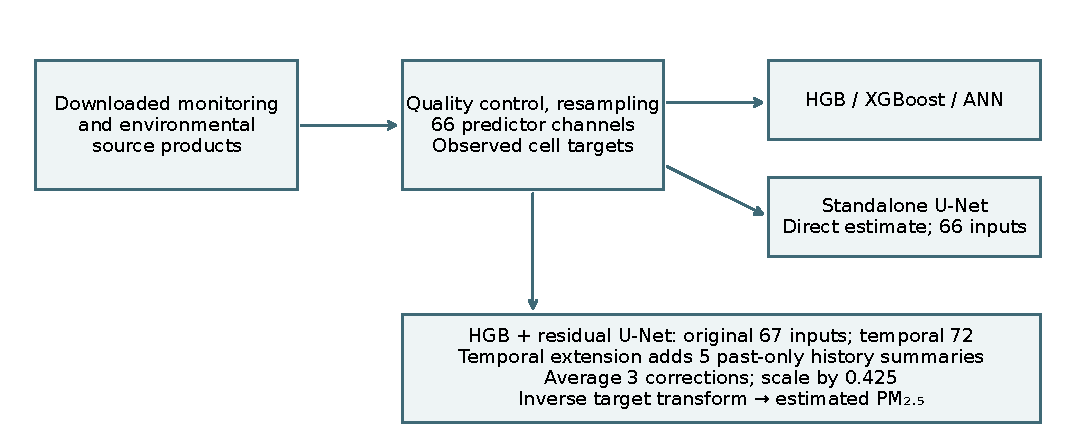
\includegraphics[width=\linewidth]{figures/pipeline.pdf}
\caption{Implemented data and model paths. The diagram describes processing
operations; it is not an experimental result. Unobserved cells do not acquire
fabricated training labels. The hybrid additionally receives the HGB baseline
map as its 67th input channel in the original configuration. The temporal
extension inserts five history channels before the HGB map, giving 72 inputs.}
\label{fig:pipeline}
\end{figure}

\subsection{Tabular boosting and ANN configurations}
HGB and XGBoost each combine a model fitted on the raw target with one fitted
in standardised log-target space. Define
\begin{equation}
 T(y)=\frac{\log(1+y)-\mu}{\sigma},\qquad
 \inv(z)=\operatorname{clip}\!\left(\exp(\mu+\sigma z)-1,0,500\right),
 \label{eq:transform}
\end{equation}
where $\mu$ and $\sigma$ are fitted using training labels. If $f_{\log}$ and
$f_{\mathrm{raw}}$ are the two predictors, their concentration-scale blend is
\begin{equation}
 \widehat y^{\mathrm{tree}}=\operatorname{clip}\!\left[
 \lambda\inv(f_{\log}(X))+(1-\lambda)
 \operatorname{clip}(f_{\mathrm{raw}}(X),0,500),0,500\right].
\end{equation}
The frozen log-model weights are 0.71 for unconstrained HGB, 0.68 for
limited-monotonic HGB and 0.83 for XGBoost. The constrained HGB makes only
the three IDW concentration-history features non-decreasing; it does not impose
monotonic effects on every environmental feature. XGBoost uses 858 log-target
trees and 115 raw-target trees, frozen from the preceding validation phase.

Both HGB variants use squared-error loss, 24 minimum samples per leaf and
no internal early stopping. The log-target member uses 350 iterations,
learning rate 0.055, 31 maximum leaf nodes and L2 regularisation 2.0; the
raw-target member uses 450 iterations, learning rate 0.05, 63 maximum leaf
nodes and L2 regularisation 3.0. The frozen XGBoost log/raw members use maximum
depths 8/6, learning rates 0.025/0.03, minimum child weights 12/8 and L2
regularisation 6.0/3.0, respectively. The stored model bundles and training
scripts retain the complete estimator configuration.

The ANN baseline is a scikit-learn multilayer perceptron with
$66\rightarrow256\rightarrow128\rightarrow1$ units, ReLU hidden activations,
Adam optimisation, regularisation parameter $10^{-4}$, learning rate
$5\times10^{-4}$ and batch size 128. It uses training-only internal early
stopping and five seeds (11, 22, 33, 44 and 55); predictions are combined across
the five fitted members. This internal stopping procedure differs from the
neural spatial models' year-based duration selection. The comparison therefore
holds observation rows and fitting years constant, but does not equalise every
training or tuning decision across model families.

\subsection{Hybrid residual U-Net}
The hybrid learns a spatial correction to unconstrained HGB in transformed
target space. With $b_t=T(\widehat y_t^{\mathrm{HGB}})$, the U-Net receives
$[X_t,b_t]$, giving 67 input channels, and predicts a residual map $r_k$ for
ensemble member $k$. The final map is
\begin{equation}
 \widehat y^{\mathrm{hybrid}}_t=
 \inv\!\left(b_t+\frac{\alpha}{3}\sum_{k=1}^{3}r_k([X_t,b_t])\right),
 \qquad \alpha=0.425.
 \label{eq:hybrid}
\end{equation}
The correction is added before the inverse transformation, not directly to
\pmfine\ concentrations. The recorded final hybrid target moments are
$\mu=2.223419$ and $\sigma=0.489477$.

The encoder widths are 32, 64 and 128, with a width-256 bottleneck. Residual
convolution blocks combine $3\times3$ convolutions, Group Normalization, SiLU
activations, spatial dropout and squeeze-and-excitation. Three decoder stages
use bilinear upsampling and concatenated encoder skips, followed by a
$1\times1$ output head. The base dropout is 0.12, scaled by depth in the code.
The output head begins at zero so that the initial hybrid estimate coincides
with its baseline. These choices specify the implemented architecture;
individual performance gains from each block have not been isolated.

For residual training, the target is $T(y_{tg})-b_{tg}$. A masked, weighted
SmoothL1 loss is used with transition parameter one:
\begin{equation}
 \mathcal L=\frac{\sum_{t,g}m_{tg}s_{tg}d(y_{tg})
   \ell_1\!\left(r_{tg}-[T(y_{tg})-b_{tg}]\right)}
 {\max(1,\sum_{t,g}m_{tg}s_{tg}d(y_{tg}))},
 \quad
 \ell_1(e)=\begin{cases}e^2/2,&|e|<1,\\|e|-1/2,&\text{otherwise}.
 \end{cases}
 \label{eq:loss}
\end{equation}
Here $d(y)$ is a training-derived density weight obtained from a
source-weighted, Gaussian-smoothed histogram and an inverse-square-root
density transformation. Scaling and clipping enforce a source-weighted mean
of one and bounds of 0.5 and 2.5. The sums in Equation~\ref{eq:loss} are
implemented over each mini-batch. No residual-magnitude penalty or raw-scale
auxiliary loss is active in this frozen configuration.

Training uses AdamW \citep{loshchilov2017}, initial learning rate
$3\times10^{-4}$, weight decay $10^{-4}$, gradient clipping at 5 and an
exponential moving average with decay 0.98. Mini-batches contain eight days,
with gradient accumulation over two batches. The final three seeds replay
validation-selected schedules: seed 42 for 16 epochs, seed 11 for 6, and seed
22 for 27. The corresponding residual predictions are averaged as in
Equation~\ref{eq:hybrid}. Training-period HGB maps are generated by an HGB
fitted on the same 2021--2023 labels. This in-sample residual-stacking design
must be distinguished from out-of-fold baseline training.

\subsection{Standalone U-Net}
The standalone model uses the same backbone pattern but receives only the
66 predictor channels. It directly estimates $T(y)$; it has no HGB input,
baseline addition or residual target. Its single-network parameter count is
1,932,481. The direct-prediction loss uses Equation~\ref{eq:loss} with
residual error replaced by $u(X)-T(y)$. Source and density weighting are
retained, with training-only preprocessing statistics.

Duration selection fits 2021--2022 and evaluates 2023 with seed 42, a maximum
of 60 epochs and patience 12. Epoch 25 and its learning-rate schedule are then
frozen. Fresh seeds 42, 11 and 22 each fit 2021--2023 for that schedule, using
batch size 8, accumulation over two batches, AdamW and EMA decay 0.98. The
standalone ensemble averages the three transformed outputs before applying
$\inv$. Seed 42 is the pre-specified single-network result. Individual seeds
11 and 22 are retained as sensitivity information, not selected as the primary
single model after viewing 2024.

\subsection{Past-only temporal extension}
\label{sec:temporal-method}
The temporal extension gives the residual network a longer description of
recent pollution without changing the U-Net backbone or the measured targets.
It adds a three-day mean, seven-day mean, seven-day maximum, seven-day standard
deviation and a recent-change feature \citep{aitkentemporal2026}. Let $h_t$
denote the prepared \texttt{pm25\_lag1\_idw\_causal} map for target day $t$.
This field already ends at day $t-1$; it is a standardised, previously clipped
predictor rather than an untransformed monitor reading. For each cell define
\begin{equation}
 \bar h^{(k)}_t=\frac{1}{n_k(t)}\sum_{j=0}^{n_k(t)-1}h_{t-j},
 \qquad n_k(t)=\min(k,t+1),\quad k\in\{3,7\},
\end{equation}
where the prepared sequence starts at index zero. The maximum and population
standard deviation use the same trailing seven-entry window. The fifth
feature is $h_t$ minus the mean of up to three preceding entries
$(h_{t-1},h_{t-2},h_{t-3})$; it is zero at the first entry. Thus the stored
``three-day trend'' is a level difference, not a fitted linear slope. Shorter
windows are used at startup, and history continues across year boundaries.

Each new channel is centred and scaled using only fitting dates and cells
inside London. Original predictors and missing-history indicators are retained.
The network input is $[X_t,H_t,b_t]$: 66 existing predictors, the five temporal
summaries $H_t$, and the HGB map, for 72 channels. The original residual loss,
backbone, seed schedules and multiplier $\alpha=0.425$ are retained. No
same-day measured \pmfine\ is added through this history construction; the
retrospective availability limits of the environmental inputs still apply.

The temporal experiment refits a common HGB baseline for its two arms rather
than reusing the original archived maps. Its raw/log blend is selected by
2023 validation RMSE and frozen for the final fit. The added summaries enter
the U-Net, not HGB. Therefore the temporal model must be compared with its
fresh matched control, not treated as a one-factor modification of the
earlier published hybrid. Both final arms use seeds 42, 11 and 22 and the
same 2021--2023 fitting window.

\section{Experimental protocol}
\subsection{Chronology and common evaluation rows}
The original development protocol uses 2021--2022 for fitting and 2023 for
external validation. The later three-year experiments refit configurations on
2021--2023 and score the available 2024 observations. The refit code does not
use 2024 labels for parameter or scaler fitting, early stopping, epoch choice,
blending or calibration. Nevertheless, earlier project runs had already
revealed 2024 results. Absence of direct fitting on those labels is therefore
not equivalent to an untouched evaluation or immunity from adaptive research
decisions.

The requested prediction interval includes all 366 days of 2024, but station
labels in the prepared package stop on 14 December. The primary common
benchmark consequently contains 9,619 LAQN station-days on 349 dates, or
95.36\% of that calendar year's days. The final 17 days are unscored; no
missing observations are generated to complete the year. Although the package
also contains 131,754 Breathe station-days in this interval, the paper's main
results refer only to LAQN. Full-grid U-Net prediction arrays cover all
366 requested dates, including unscored dates.

\subsection{Temporal comparison and model status}
The temporal experiment first fits 2021--2022 and evaluates 11,102 LAQN
station-days in 2023. Its pre-written promotion rule requires lower overall
RMSE, higher $R^2$, lower high-concentration MAE, non-increasing MAE below
15~\ug, and signed bias below 15~\ug\ no greater than
$\max(0.10,\text{control bias})$. It improves the error measures slightly but
increases that bias from $+0.3892$ to $+0.4024$~\ug, missing the guard by
0.0132~\ug. Despite this, the saved experiment subsequently evaluates both
three-seed final fits on 2024. That comparison is an exploratory retrospective
result, not a validation-approved promotion or an untouched confirmation.
The original hybrid remains the official model.

\subsection{Metrics and descriptive uncertainty}
For station observations $y_i$, predictions $p_i$ and errors $e_i=p_i-y_i$,
the primary metrics are
\begin{equation}
 \mathrm{MAE}=\frac{1}{N}\sum_i|e_i|,\quad
 \mathrm{RMSE}=\sqrt{\frac{1}{N}\sum_i e_i^2},\quad
 R^2=1-\frac{\sum_i e_i^2}{\sum_i(y_i-\bar y)^2}.
\end{equation}
Mean error reports bias. These are pooled station-day metrics, so stations with
more available days have greater representation. $R^2$ is not a percentage
accuracy. Within-day spatial correlation is calculated after subtracting each
day's observed and predicted station means and pooling the centred values on
days with at least three stations. It assesses relative within-day variation
at monitors rather than agreement at unmonitored cells.

High-concentration diagnostics use $y_i\geq25$~\ug, a project-defined analysis
threshold, not a claimed regulatory or health standard. The benchmark has
216 such rows. The saved comparison audit also provides 50,000 paired
calendar-day bootstrap repetitions. Each resample preserves the paired models
and all station rows within a sampled day; RMSE is recomputed on the sampled
rows. Reported intervals are the 2.5th and 97.5th percentiles of model
differences. They are descriptive, post-selection and unadjusted for multiple
comparisons. Resampling whole days retains within-day clustering but does not
model serial dependence across successive dates. Separately, the temporal
report provides a paired seven-calendar-day block-bootstrap RMSE-difference
interval, retaining short-range temporal grouping as well as paired rows.
That interval and the original single-day intervals are distinct analyses and
are labelled separately. Neither accounts for prior benchmark inspection or
establishes uncertainty in predictions at unmonitored cells.

\subsection{Artifact verification}
The original comparison tables and performance figures are generated from the
saved station prediction table. The accompanying script checks the 9,619 unique
station-day keys, date coverage and finite values, and independently recomputes
MAE, RMSE, $R^2$, bias, high-event errors and centred spatial correlation.
Recomputed metrics agree with the saved experiment metrics within $10^{-6}$.
File hashes record the input artifacts. Bootstrap intervals are transcribed
from the final saved audit, rather than recomputed during manuscript
preparation. These checks establish consistency of saved artifacts and
arithmetic; they are not a new end-to-end retraining or independent validation
of every provider measurement.

Temporal results are transcribed from the versioned metrics CSV, report and
audit \citep{aitkentemporal2026}. The prior audit records recalculated metrics,
identical evaluation rows, unchanged source inputs and hashes of all six final
checkpoints. Those temporal prediction arrays and checkpoints are not available
locally for this manuscript update. We therefore verify the aggregate values,
differences and source-file hashes, but do not claim to rerun the temporal
audit or its bootstrap. Temporal station-level plots and spatial correlations
are not inferred from aggregate scores.

\section{Results}
\subsection{Common-benchmark performance}
The temporal hybrid has the lowest recorded MAE and RMSE in
Table~\ref{tab:main}; the matched comparison is detailed in
Section~\ref{sec:temporal-results}. Within the original configurations,
the hybrid's RMSE is 3.7765~\ug, compared with
3.7920~\ug\ for unconstrained HGB, a relative reduction of approximately
0.41\%. The small difference is visible against the broader configuration
spread in Figure~\ref{fig:ranking}. The models are close enough that the
distinction between numerical ranking and evidence of a reliable advantage
matters.

\begin{table}[tb]
\caption{Common LAQN benchmark: 9,619 station-days, 1 January--14 December 2024;
final fitting on 2021--2023. MAE and RMSE are in \ug. The later temporal
comparison uses its own matched HGB refit. Bold identifies the best scores
within each group, not statistical significance or model promotion.}
\label{tab:main}
\centering\small
\begin{tabular}{@{}lrrr@{}}
\toprule
Configuration & MAE $\downarrow$ & RMSE $\downarrow$ & $R^2$ $\uparrow$ \\
\midrule
\multicolumn{4}{@{}l}{\textit{Original archived configurations}}\\
\tableinput{tables/main_results.tex}
\midrule
\multicolumn{4}{@{}l}{\textit{Later matched temporal comparison (experimental)}}\\
\tableinput{tables/temporal_results.tex}
\bottomrule
\end{tabular}
\end{table}

\begin{figure}[tb]
\centering
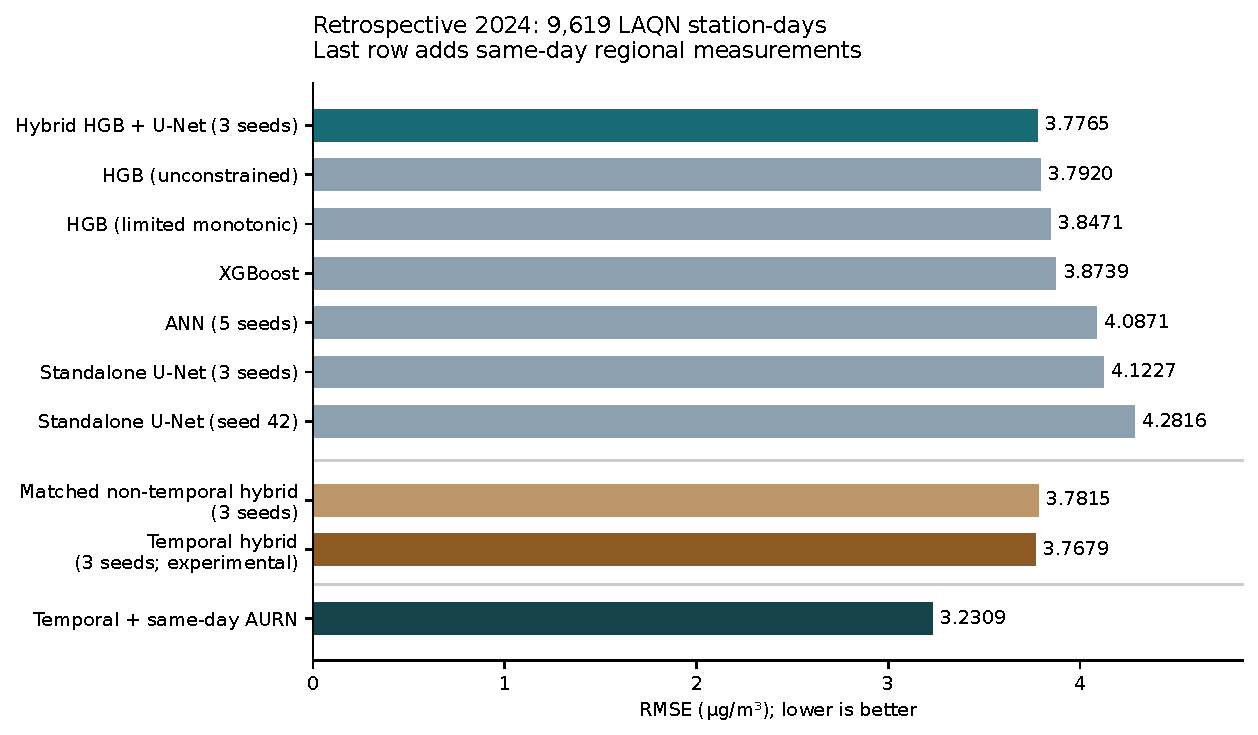
\includegraphics[width=.94\linewidth]{figures/rmse_comparison.pdf}
\caption{Original RMSE values recomputed from saved predictions, with the
two later temporal-comparison values transcribed from the saved audit.
All score 9,619 LAQN rows. The horizontal axis starts at zero. Bars show point
estimates, not uncertainty, computational cost or deployment status.}
\label{fig:ranking}
\end{figure}

The standalone ensemble reaches RMSE 4.1227~\ug, exceeding both HGB and the
hybrid. Its pre-specified single member, seed 42, reaches 4.2816~\ug.
The other two single networks obtain 4.1973 (seed 11) and 4.0692~\ug\
(seed 22). Reporting the lower seed-22 result as a pre-selected best standalone
model would use evaluation outcomes to choose the model. These results
characterise the tested training recipe and do not establish the best
performance attainable by every standalone U-Net.

The tabular baselines also show metric-dependent ordering. XGBoost has lower
MAE than limited-monotonic HGB but higher RMSE. The ANN has higher RMSE than
the tree configurations, while its RMSE is slightly below the standalone
U-Net ensemble. Thus, a single statement that all neural models outperform
all tree models would contradict the observed results.

\subsection{Latest temporal result and its matched comparison}
\label{sec:temporal-results}
The temporal hybrid obtains MAE 2.3361~\ug, RMSE 3.7679~\ug\ and
$R^2=0.5201$. Its freshly fitted non-temporal control obtains 2.3443~\ug,
3.7815~\ug\ and 0.5166, respectively. The matched RMSE reduction is
0.0136~\ug\ (approximately 0.36\%), with MAE lower by 0.0082~\ug\ and
$R^2$ higher by 0.0035. The saved paired seven-day-block interval for
temporal-minus-control RMSE is [$-0.0203$, $-0.0075$]~\ug. This describes
a small retrospective gain in this experiment, not a prospective superiority
claim. It is not an interval for comparison with the original 3.7765~\ug\
hybrid or with HGB alone.

\begin{table}[tb]
\caption{Temporal comparison on the same 2024 observations. All values are
in \ug; concentration bands are defined by observed values. Both models
remain strongly biased low on high-concentration observations.}
\label{tab:temporal-diagnostics}
\centering\small
\begin{tabular}{@{}lrr@{}}
\toprule
Diagnostic & Matched control & Temporal hybrid \\
\midrule
\tableinput{tables/temporal_diagnostics.tex}
\bottomrule
\end{tabular}
\end{table}

The high-concentration MAE falls only from 14.1090 to 14.0490~\ug
(Table~\ref{tab:temporal-diagnostics}). Thus the lower overall RMSE does not
resolve the dominant episode-error problem. The temporal configuration is
the best recorded numerical result, but is retained as experimental because
it did not pass the earlier 2023 promotion guard. This qualification is part
of interpreting its favourable 2024 scores, not a reason to discard those scores.

\subsection{Magnitude and uncertainty of the original hybrid improvement}
Table~\ref{tab:bootstrap} reports the saved paired-day bootstrap comparisons
for the original five-configuration refit. For unconstrained HGB, the RMSE
difference is 0.01548~\ug. Its descriptive interval runs from $-0.00003$ to
$0.02830$~\ug. The intervals for
limited-monotonic HGB and XGBoost also include zero. These intervals do not
establish a clear RMSE advantage of the hybrid over those alternatives, but
neither do they prove equivalence. The ANN interval excludes zero in this
descriptive analysis; it remains subject to the same post-selection and
dependence limitations.

\begin{table}[tb]
\caption{Saved descriptive paired-day bootstrap results: candidate RMSE minus
hybrid RMSE, in \ug. Positive differences favour the hybrid. The near-zero HGB
endpoint is shown to five decimals to avoid hiding its negative sign.}
\label{tab:bootstrap}
\centering\small
\begin{tabular}{@{}lrl@{}}
\toprule
Candidate & Difference & Descriptive 95\% interval \\
\midrule
\tableinput{tables/bootstrap.tex}
\bottomrule
\end{tabular}
\end{table}

The later standalone audit reports a standalone-ensemble-minus-HGB RMSE
difference of 0.3306~\ug\ with descriptive interval [0.0926, 0.5712]~\ug,
and a standalone-minus-hybrid difference of 0.3461~\ug\ with interval
[0.1029, 0.5908]~\ug. These use the same day-resampling approach and do not
convert the retrospective comparison into a confirmatory hypothesis test.

\subsection{Spatial variation and high-concentration errors}
All reported configurations have negative mean error
(Table~\ref{tab:diagnostics}). The original hybrid's within-day spatial correlation is
0.6537, above unconstrained HGB's 0.6337, but below limited-monotonic HGB's
0.6579. This shows that the model with the lowest pooled RMSE does not lead
every spatial diagnostic. The correlations remain measurements at available
stations, with no implication that each intervening grid cell is validated.

\begin{table}[tb]
\caption{Original-configuration diagnostic results on the same LAQN rows. Bias and high-concentration
MAE are in \ug. High-concentration MAE uses the 216 observations with measured
\pmfine\ at least 25~\ug; spatial $r$ is pooled within-day-centred correlation.}
\label{tab:diagnostics}
\centering\small
\begin{tabular}{@{}lrrr@{}}
\toprule
Configuration & Bias & Spatial $r$ $\uparrow$ & High MAE $\downarrow$ \\
\midrule
\tableinput{tables/diagnostics.tex}
\bottomrule
\end{tabular}
\end{table}

High-concentration error remains substantial for the hybrid and HGB, at
14.0668 and 14.2033~\ug\ MAE, respectively. These 216 rows represent only
2.25\% of the benchmark but account for approximately 39.0\% of HGB's total
squared error. The parity plots in Figure~\ref{fig:parity} show the compression
of predictions at higher observed concentrations. The standalone ensemble has
high-concentration MAE 16.2035~\ug. Its threshold recall is 1/216 (0.46\%),
whereas HGB and the hybrid each flag 12/216 (5.56\%) of these observed high
rows at the same threshold. These are retrospective threshold diagnostics,
not a deployed event-warning evaluation.

\begin{figure}[tb]
\centering
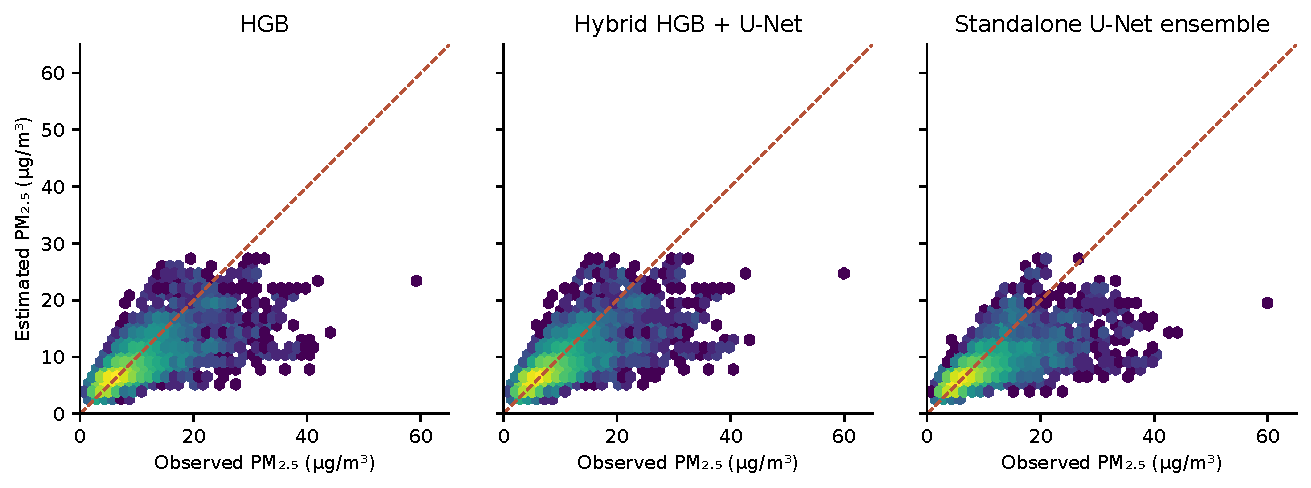
\includegraphics[width=\linewidth]{figures/parity.pdf}
\caption{Saved station predictions against measured \pmfine\ for three
original configurations, not the temporal extension, on all 9,619 common rows.
Hexagonal bins use logarithmic counts
to reveal concentration density; colour intensities are independently
normalised per panel and are not compared across panels. Axes are common and
the dashed line denotes perfect agreement. These are station comparisons,
not full-grid ground-truth maps.}
\label{fig:parity}
\end{figure}

\FloatBarrier
\section{Discussion and limitations}
\subsection{What the model comparison establishes}
The results support retaining HGB as a strong reference for this problem and
describing the hybrid as a modest numerical refinement. The U-Net correction
can use neighbouring predictor patterns, but the baseline already incorporates
coordinates, environmental information and prior-day IDW fields. Limited
additional information after baseline fitting is a plausible explanation for
the small gain; it is an interpretation, not a demonstrated causal mechanism.
The additional temporal summaries give a further small matched gain, while
leaving high-concentration errors largely unresolved. No controlled ablation
isolates the contribution of every input group,
architectural block, ensemble size or training-loss choice in the final
three-year experiment.

The standalone comparison is informative but not a pure one-factor ablation
of the HGB input. Removing HGB also changes the learning target from a residual
to a direct prediction, and the frozen training durations differ. Similarly,
the three-seed spatial models and five-seed ANN do not have matched ensemble
budgets. The study does not measure inference latency, energy use or a
controlled cost--accuracy trade-off. A preference for the simpler HGB pipeline
is therefore a design judgement supported by close error scores, not a measured
runtime superiority claim.

\subsection{Temporal evaluation and information availability}
Prior inspection of 2024 is the main barrier to a prospective performance
claim. Preserving frozen refit scripts and hashes prevents silent changes to
the reported configurations but cannot erase knowledge gained from previous
evaluation runs. A future untouched period or nested rolling-origin protocol
is required to assess robustness to research decisions and temporal change.
The present package also leaves the last 17 days of 2024 unscored.

Operational availability is a second, separate constraint. Same-day ERA5
reanalysis and same-quarter Sentinel-2 composites are appropriate for
retrospective reconstruction, but may be unavailable at a real forecast issue
time. Census and emissions inventories are static reference products rather
than contemporaneous daily observations. A deployment-oriented evaluation
would need covariates available by a specified issue time, archived forecast
weather and explicitly lagged satellite composites. No such evaluation is
reported here.

\subsection{Spatial supervision and source dependence}
The benchmark evaluates temporal behaviour at available regulatory stations;
it is not a geographically blocked holdout. Earlier observations from the
same sites can influence later IDW predictors. Some station-day observations
also share grid cells, so row count is not a count of independent spatial
locations. The 1,719-cell prediction domain and visually smooth maps do not
provide full-grid truth. Regional transfer, accuracy at previously unmonitored
locations and improvement at specific neighbourhoods remain unestablished.

Breathe observations provide much of the training coverage, but source
weighting does not establish that their residual errors are negligible. Their
documented reference-network correction also means that sensor provenance
should not be treated as wholly independent of LAQN. This study does not
independently audit the timing or reference data used by the upstream sensor
calibration system, and therefore does not make an end-to-end independence
claim. The 4:1 mixed-cell target and 0.15 Breathe-only training weight are
specific modelling decisions, not universally validated reliability ratios.

\subsection{Stacking, preprocessing and statistical limits}
In-sample HGB predictions used during residual training can differ in error
distribution from predictions on later data. An out-of-fold or time-blocked
baseline would better align residual training with generalisation error.
The current design contains no direct 2024-label fitting in the refit, but
this does not remove the stacking limitation. Likewise, normalising the
existing float16 cube preserves its earlier clipping and quantisation.

The original day-level bootstrap omits across-day serial dependence. The
temporal comparison's seven-day blocks address short-range dependence, but
neither analysis corrects for multiple comparisons or benchmark inspection.
Intervals near zero should be interpreted cautiously, and they are not
spatial uncertainty bands for the output maps. High-event underprediction is
observed, but attribution to log targets, robust loss, density weighting,
distribution shifts or smooth covariates would require additional controlled
experiments. These possibilities are hypotheses for follow-up work.

\section{Conclusion}
A completed multi-source Greater London pipeline enables a transparent
comparison of daily \pmfine\ estimation configurations on a shared regulatory
benchmark. The best recorded experimental configuration is the temporal
HGB--residual-U-Net ensemble: MAE 2.3361~\ug, RMSE 3.7679~\ug\ and
$R^2=0.5201$ on 9,619 station-days. Against its matched non-temporal control,
the RMSE reduction is 0.0136~\ug\ (0.36\%), with descriptive seven-day-block
interval [$-0.0203$, $-0.0075$]~\ug\ for temporal minus control. This small
retrospective improvement does not meet the separate 2023 validation bias
guard, so the original hybrid remains the official model. Its RMSE is
3.7765~\ug, compared with HGB's 3.7920~\ug\ and the tested standalone
U-Net ensemble's 4.1227~\ug. Peak errors remain substantial even for the
temporal hybrid, with high-concentration MAE 14.0490~\ug.

The findings justify a bounded conclusion about this implementation and
benchmark, not a claim of general U-Net superiority, state-of-the-art
performance, operational forecasting or validated accuracy throughout every
grid cell. The next substantive evaluation should combine an untouched time
period, spatially blocked assessment, issue-time-available covariates and
out-of-fold residual baselines. Those are proposed experiments and are not
reported as completed work.

\section*{Data and code availability}
This manuscript is based on the local \texttt{pm25\_london\_bundle} implementation
and its saved experiment artifacts. The accompanying manuscript package
includes LaTeX source, bibliography, generated tables, figures, the asset
generation script and an evidence manifest. Raw data, fitted model binaries
and the full processed cube are not bundled with the manuscript. Provider
references identify the original sources; Breathe API access requires an
appropriate key. Project code and curated result reports are maintained in
\href{https://github.com/r9jdp/Aitken}{the Aitken repository}; the temporal
experiment and aggregate audit are identified in \citet{aitkentemporal2026}.
The maintained manuscript source is in \texttt{research\_paper} within that
repository. No archived data DOI or unrestricted raw-data redistribution
licence is claimed. Provider terms and data access remain separate from code
availability.

\bibliographystyle{unsrtnat}
\bibliography{references}

\clearpage
\appendix
\section{Artifact provenance and reproduction}
The paper is based on completed saved runs, rather than newly trained models.
Within \texttt{code/pm25\_london\_bundle/artifacts}, the principal directories are:
\begin{itemize}
\item \nolinkurl{london_3year_tree_refit_20260905_141738}: HGB and XGBoost refits.
\item \nolinkurl{london_3year_unet_refit_20260905_142452}: hybrid refit.
\item \nolinkurl{london_exact_sklearn_ann_train2021_2023_test2024}: ANN refit.
\item \nolinkurl{london_3year_final_comparison_20260905_145050}: original common
comparison, metrics and final bootstrap audit.
\item \nolinkurl{london_standalone_unet_20260906}: standalone experiment and
extended common prediction table.
\end{itemize}
The paper's \nolinkurl{build_assets.py} recomputes its tables from the last
directory's \nolinkurl{test_2024_laqn_all_models.csv.gz}. The original
five-model comparison supplies the bootstrap table. Input SHA-256 values and
verification scope are recorded in \nolinkurl{evidence/provenance.json};
unrounded recomputed values appear in \nolinkurl{evidence/recomputed_metrics.csv}.
Run \texttt{py -3.10 research\_paper/build\_assets.py} from the Aitken repository
root to regenerate the original comparison assets. An explicit
\texttt{--bundle} path can point to the read-only original London bundle.
The script also generates the temporal table from
\nolinkurl{results/temporal_model_20260912/metrics.csv}, checks the recorded
\nolinkurl{audit.json}, and records those files and \nolinkurl{REPORT.md}
in \nolinkurl{evidence/temporal_provenance.json}. The
\texttt{--temporal-only} option refreshes only the temporal tables and
provenance without requiring the large original artifacts. Neither mode
retrains models. The seven-day temporal interval is transcribed from the
versioned report; it is not substituted for the original day-level intervals.

The handoff records a Python 3.10.5 environment with PyTorch 2.10.0+cu126,
scikit-learn 1.7.2, XGBoost 3.1.2 and NumPy 2.2.6. These are recorded project
environment versions, not a claim that the manuscript independently rebuilt
each model in that environment. Full refit commands and preprocessing
provenance remain in the model directories and project handoff.

\section{Ordered retained feature schema}
\label{app:features}
The following names are copied from the actual prepared schema after removing
the five fire/smoke channels. There are 66 retained channels; the hybrid
concatenates its separately generated HGB map as channel 67.

The temporal extension inserts the following ordered channels before HGB:
\begin{enumerate}[start=67]
\item \texttt{history\_mean\_3d}
\item \texttt{history\_mean\_7d}
\item \texttt{history\_max\_7d}
\item \texttt{history\_std\_7d}
\item \texttt{history\_trend\_3d}
\end{enumerate}
Its separately generated HGB map is channel 72. The table below lists the
unchanged 66 predictors shared with the original configurations.
\footnotesize
\begin{longtable}{@{}rl@{}}
\caption{Retained predictor channels in model order.}\label{tab:features}\\
\toprule
Index & Stored feature name \\
\midrule
\endfirsthead
\toprule
Index & Stored feature name (continued) \\
\midrule
\endhead
\bottomrule
\endfoot
\tableinput{tables/feature_names.tex}
\end{longtable}
\normalsize

% Editorial review is supplied separately in REVIEW_AND_CLAIMS.md so that
% revision questions do not masquerade as scientific results in the paper.
\end{document}
